\documentclass{article}

\usepackage[utf8x]{inputenc}
\usepackage[english,russian]{babel}
\usepackage{graphicx}
\usepackage{amsmath}
\usepackage{amssymb}
\usepackage{extarrows}
\usepackage{vmargin}
\usepackage{MnSymbol}
\setpapersize{A4}
\setmarginsrb{2cm}{2cm}{2cm}{2cm}{0pt}{0mm}{0pt}{13mm}

%user commands
\newtheorem{theorem}{Теорема}
\newtheorem{lemma}{Лемма}

\newenvironment{proof}{\paragraph{Доказательство:}}{\hfill$\blacksquare$}
\newenvironment{definition}{ \paragraph{Определение:}}{\hfill $\blacktriangleleft$}
\newenvironment{observation}{ \paragraph{Замечание:}}{\\}
\newenvironment{hence}{ \paragraph{Следствие:}}{}


\begin{document}

\centerline{\large Курс лекция для магистров ВМК МГУ}
\centerline {\textbf{\LARGE Обратные задачи математической физики}}
\centerline {Затехал Строков Вениамин 2025}

\vspace{0.4cm}

\centerline{\LARGE 	Лекция 4. Обратные задачи для уравнения теплопроводности}
\centerline{\LARGE 	в неограниченных областях}

\vspace{0.5cm}
\centerline{\large Задача об определении источника тела}

\begin{equation*}
\begin{cases}
	u_t = u_{xx} + f(x) g(t), & 0 < x < l, 0 < t < T;\\
	u(x,0) = 0;\\
	u_x(0,t) = u_x(l,t), & 0 \leqslant t \leqslant T.
\end{cases}
\end{equation*}

Была рассмотрена такая ОЗ, когда $g(t) $ известна, требовалось найти $f(x)$  по $u(x_0,t)$.
Единственность существенно зависела от выбора точки $x_0$. 
Необходимое условие было $cos(\dfrac{\pi n x_0}{l}) \neq 0$. 
В случае известного $f(x)$ была доказана единственность определения $g(t)$ при $f(x_0) \neq 0$.
 
Рассмотрим случай бесконечной прямой:
\begin{equation*}
\begin{cases}
	u_t = u_{xx} + f(x) g(t), & -\infty < x < \infty, 0 < t < T;\\
	u(x,0) = 0;\\
	|u(x,t)| \leqslant M.
\end{cases}
\end{equation*}

ОЗ1 - дано: $g(t)$, $u(0,t) = h(t)$, $0 < t_0 \leqslant t \leqslant t_1$. 
Найти $f(x)$: $|f(x)| \leqslant M$.

Построим решение Прямой Задачи, пусть $g(t) \equiv 1$
\begin{equation*}
u(x,t) = \int_0^t \int_{-\infty}^{\infty} \dfrac{e^{\frac{-(x-\xi)^2}{4(t-\tau)}}}{\sqrt{4 \pi (t -\tau)}}  f(\xi) d\xi d \tau.
\end{equation*}

Положим $x = 0$, получим уравнение относительно $f(x)$:
\begin{equation*}
	h(t) = \int_0^t \int_{-\infty}^{\infty} \dfrac{e^{\frac{-\xi^2}{4(t-\tau)}}}{\sqrt{4 \pi (t -\tau)}}  f(\xi) d\xi d \tau = 
	\{ G(\xi,\theta) = \dfrac{e^{\frac{-\xi^2}{4 \theta}}}{\sqrt{4 \pi \theta}} \} =
	\int_0^t \int_{-\infty}^{\infty} G(\xi, \theta) f(\xi) d\xi d \theta,
 	\hspace{0.5cm} t_0 \leqslant t \leqslant t_1.
\end{equation*}

Исследуем единственность решения ОЗ1, положив $h=0$ на $[t_0,t_1] \subset [0,T]$
\begin{equation*}
	\int_0^t \int_{-\infty}^{\infty} G(\xi, \theta) f(\xi) d\xi d \theta = 0,
 	\quad t_0 \leqslant t \leqslant t_1
\end{equation*}

\begin{equation}
	\dfrac{\partial}{\partial t}: \quad
	\int_{-\infty}^{\infty} G(\xi, \theta) f(\xi) d\xi = 0,
 	\quad t_0 \leqslant t \leqslant t_1
	\label{partial of int}
\end{equation}

Рассмотрим вспомогательную задачу
\begin{equation*}
\begin{cases}
	v_t = v_{xx}, & -\infty < x < \infty, 0 < t;\\
	v(x,0) = f(x).
\end{cases}
\end{equation*}

\begin{equation}
	v(x,t) = \dfrac{1}{\sqrt{4 \pi t}} \int_{-\infty}^{\infty} f(\xi) e^{\frac{-(x-\xi)^2}{4t}} d\xi = 
	\int_{-\infty}^{\infty} G(x-\xi, t) f(\xi) d\xi.
	\label{v(x,t)}
\end{equation}

% To do. сделать нормальные ссылки
Положим $x = 0$. Тогда из (\ref{partial of int}) и (\ref{v(x,t)}) имеем
\begin{equation}
	v(0,t) = \int_{-\infty}^{\infty} G(\xi, t) f(\xi) d\xi
 	\quad t_0 \leqslant t \leqslant t_1
 	\label{v(0,t)}
\end{equation}

Покажем, что (\ref{v(0,t)}) $\Rightarrow f(x) = 0, \forall x \in \mathbb{R}$
Введём $F(z) = \int_{-\infty}^{\infty} \dfrac{e^{\frac{-\xi^2}{4z}}}{\sqrt{4 \pi z}} f(\xi) d\xi$ для $Re z \geqslant \varepsilon > 0$.
 $F(z)$ аналитична и  при $Im z = 0, Re z \in [t_0,t_1] \Rightarrow$ $F(z) = 0$ при $Re z \geqslant \varepsilon > 0$, но тогда $F(z) = 0$ при $Re z > 0$, т.е. при $t>0$.
\begin{equation*}
	v(0,t) = \int_{-\infty}^{\infty} G(\xi, t) f(\xi) d\xi = 0.
\end{equation*}
 
\vspace{0.2cm}
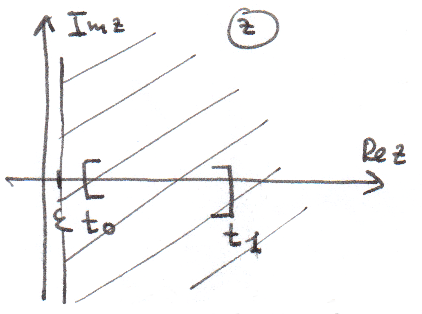
\includegraphics[scale=0.85]{pic4_1.png}
\vspace{0.2cm}


Таким образом, 
$
\int_{-\infty}^{\infty} e^{\frac{-\xi^2}{4t}} f(\xi) d\xi = 0, t \geqslant 0,
$
поскольку $v(x,t)$ - решение задачи Коши и $v(0, +0) = v(0,0) = f(x) = 0$.
Сделаем замену $\{ \xi^2 = s$, $\xi = \sqrt{s} \}$, и заметим, что если $f(x)$ - не чётна, то 
$
\int_{-\infty}^{\infty} e^{\frac{-\xi^2}{4t}} f(\xi) d\xi = 0
$.
Поэтому считаем пока, что $f(x)$ - чётна 
$
\Rightarrow \int_0^{\infty} e^{\frac{-s}{4t}} \dfrac{f(\sqrt{s})}{\sqrt{s}} d s \neq 0, \forall t > 0
$.
Но это преобразование Лапласа функции $f(\sqrt{s}) / \sqrt{s}$ с параметром $1 / (4t)$. В силу взаимно-однозначности (теорема Лёрха) $f(\sqrt{s})  = f(\xi) = 0$ при $\xi \geqslant 0$.
Таким образом, справедлива теорема единственности.

\begin{theorem}
	Пусть $|f(x)| < M$ и $f(x)$ - чётная. Тогда $u(0,t)$, $t \in[t_0,t_1]$ однозначно определяет $f(x)$
\end{theorem}

Для нахождения $f(x)$ можно использовать уравнение 
\begin{equation*}
	\int_{-\infty}^{\infty} K(x,t) f(x) dx = h(t),
	\quad t_0 \leqslant t \leqslant t_1,
\end{equation*}

где 
\begin{equation*}
	K(x,t) = \int_0^t \dfrac{e^{\frac{-x^2}{4 (t-\tau)}}}{\sqrt{4 \pi (t -\tau)}}  g(\tau) d \tau.
\end{equation*}

\begin{hence}
	Если известны $u(0,t)$ и $u_x(0,t)$  при $[t_0,t_1]$, тогда $f(x)$ определяется однозначно.
\end{hence}

Рассмотрим ОЗ2:

$f(x)$ известна, дано $u(0,t) = h(t), t\in [0,T]$,  найти $g(t)$.

Получим уравнение ОЗ:
\begin{align*}
	u(0,t) =& \int_0^t \int_{-\infty}^{\infty} \dfrac{e^{\frac{-\xi^2}{4 (t-\tau)}}}{\sqrt{4 \pi (t -\tau)}} f(\xi) g(\tau) d \xi d \tau = \\
	= h(t) =&
	\int_0^t g(\tau) \int_{-\infty}^{\infty} \dfrac{e^{\frac{-\xi^2}{4 (t-\tau)}}}{\sqrt{4 \pi (t -\tau)}} f(\xi)  d \xi d \tau =
	\int_0^t g(\tau) v(0,t-\tau) d \tau
	, \quad t \in[0,T]
\end{align*}

или
\begin{equation}
	\int_0^t K(t-\tau) g(\tau) d \tau = h(t)
	\label{h(t)}
\end{equation}
где
\begin{equation}
	K(t-\tau	) = K(\theta) = 
	\int_{-\infty}^{\infty} \dfrac{e^{\frac{-\xi^2}{4 \theta}}}{\sqrt{4 \pi \theta}}  f(\xi) d \xi = v(0,\theta),
	\label{K(theta)}
\end{equation}
\begin{equation*}
	K(0) = v(0,0) = f(0).
\end{equation*}

Уравнение (\ref{h(t)}) - уравнение Вольтерра I рода. 
Сведём его к уравнению II рода.
Продифференцируем (\ref{h(t)})
\begin{equation}
	K(0) g(t) + \int_0^t K'(t-\tau) g(\tau) d \tau = h'(t), 
	\hspace{0.5cm} t \in [0,T].
	\label{K(0) g(t)}
\end{equation}

\begin{theorem}
	(Существования и единственности)
	Пусть $f \in C^2(\mathbb{R})$, $|f|, |f''| < M$ на $\mathbb{R}$ и $f(0) \neq 0$.
	Тогда, если $h \in C^1[0,T]$ и $h(0) = 0$, то решение ОЗ2 существует и единственно
\end{theorem}
\begin{proof}

Докажем что $K(\theta)$ из (\ref{K(theta)}) непрерывно Дифференцируема на $[0,T]$. 
Очевидно что достаточно исследовать дифференцируемость в нуле. 
Рассмотри вспомогательную задачу:
\begin{equation*}
\begin{cases}
	\omega_t = \omega_{xx},& -\infty < x < \infty, t> 0;\\
	\omega(x,0) = f''(x).
\end{cases}
\end{equation*}

Тогда 
\begin{equation*}
	\omega(x,t) = \dfrac{1}{\sqrt{4 \pi t}} \int_{-\infty}^{\infty} f''(\xi) e^{\frac{-(x-\xi)^2}{4 \pi t}} d\xi,
\end{equation*}

и $\omega(x,t) = v_{xx} (x,t)$, поскольку интеграл для $\omega(x,t)$ сходится равномерно по $x$, а сверка обладает свойством 
\begin{equation*}
	\int_{-\infty}^{\infty} f(\xi) e^{-\alpha(x - \xi)^2} d\xi = 
	\int_{-\infty}^{\infty} f(x -\xi) e^{-\alpha \xi^2} d\xi
\end{equation*}

Следовательно, $\omega = v_{xx} = v_t(x,t)$, но поскольку $\omega \in C(\mathbb{R} \times [0,T])$, то $v_t(0,t) \in C[0,T]$.
Таким образом, $K'(\theta) \in C[0,T] $. Кроме того, $K(0) = K(0,0) = f(0) \neq 0$. 
Следовательно (\ref{K(0) g(t)}) интегральное уравнение Вольтерра II рода имеет единственное решение.

\end{proof}





\end{document}